%%%%% Set up %%%%%

% Set document style and font size
\documentclass[12pt]{article}\usepackage[]{graphicx}\usepackage[]{color}
%% maxwidth is the original width if it is less than linewidth
%% otherwise use linewidth (to make sure the graphics do not exceed the margin)
\makeatletter
\def\maxwidth{ %
  \ifdim\Gin@nat@width>\linewidth
    \linewidth
  \else
    \Gin@nat@width
  \fi
}
\makeatother

\definecolor{fgcolor}{rgb}{0.345, 0.345, 0.345}
\newcommand{\hlnum}[1]{\textcolor[rgb]{0.686,0.059,0.569}{#1}}%
\newcommand{\hlstr}[1]{\textcolor[rgb]{0.192,0.494,0.8}{#1}}%
\newcommand{\hlcom}[1]{\textcolor[rgb]{0.678,0.584,0.686}{\textit{#1}}}%
\newcommand{\hlopt}[1]{\textcolor[rgb]{0,0,0}{#1}}%
\newcommand{\hlstd}[1]{\textcolor[rgb]{0.345,0.345,0.345}{#1}}%
\newcommand{\hlkwa}[1]{\textcolor[rgb]{0.161,0.373,0.58}{\textbf{#1}}}%
\newcommand{\hlkwb}[1]{\textcolor[rgb]{0.69,0.353,0.396}{#1}}%
\newcommand{\hlkwc}[1]{\textcolor[rgb]{0.333,0.667,0.333}{#1}}%
\newcommand{\hlkwd}[1]{\textcolor[rgb]{0.737,0.353,0.396}{\textbf{#1}}}%
\let\hlipl\hlkwb

\usepackage{framed}
\makeatletter
\newenvironment{kframe}{%
 \def\at@end@of@kframe{}%
 \ifinner\ifhmode%
  \def\at@end@of@kframe{\end{minipage}}%
  \begin{minipage}{\columnwidth}%
 \fi\fi%
 \def\FrameCommand##1{\hskip\@totalleftmargin \hskip-\fboxsep
 \colorbox{shadecolor}{##1}\hskip-\fboxsep
     % There is no \\@totalrightmargin, so:
     \hskip-\linewidth \hskip-\@totalleftmargin \hskip\columnwidth}%
 \MakeFramed {\advance\hsize-\width
   \@totalleftmargin\z@ \linewidth\hsize
   \@setminipage}}%
 {\par\unskip\endMakeFramed%
 \at@end@of@kframe}
\makeatother

\definecolor{shadecolor}{rgb}{.97, .97, .97}
\definecolor{messagecolor}{rgb}{0, 0, 0}
\definecolor{warningcolor}{rgb}{1, 0, 1}
\definecolor{errorcolor}{rgb}{1, 0, 0}
\newenvironment{knitrout}{}{} % an empty environment to be redefined in TeX

\usepackage{alltt}

% File path to resources (style file etc)
\newcommand{\locRepo}{csas-style}

% Style file for DFO Technical Reports
\usepackage{\locRepo/tech-report}

% header-includes from R markdown entry
\usepackage{pdflscape}

%%%%% Variables %%%%%

% New definitions: Title, year, report number, authors
% Protect lower case words (i.e., species names) in \Addlcwords{}, in "TechReport.sty"
\newcommand{\trTitle}{Development of methods in support of a head-only catch sampling program for sablefish (\emph{Anoplopoma fimbria}) in British Columbia}
\newcommand{\trYear}{2022}
\newcommand{\trReportNum}{nnn}
% Optional
\newcommand{\trAuthFootA}{Email: \link{mailto:Lacko.Lisa@dfo-mpo.gc.ca}{\nolinkurl{Lacko.Lisa@dfo-mpo.gc.ca}} \textbar{} telephone: (778) 268-3236}
\newcommand{\trAuthsLong}{Lisa C. Lacko and Kathryn L. Temple and Kendra R. Holt and Janine x. Supernault}
\newcommand{\trAuthsBack}{L.C. Lacko, Kathryn L. Temple and Holt K.R. and Supernault J.x.}

% New definition: Address
\newcommand{\trAddy}{Pacific Biological Station\\
Fisheries and Oceans Canada, 3190 Hammond Bay Road\\
Nanaimo, British Columbia, V9T 6N7, Canada\\}

% Abstract
\newcommand{\trAbstract}{Routine biological sampling of whole round sablefish from commercial fishing operations in British Columbia began the early 1990's. Historically, specimens were obtained through the voluntary fishery catch sampling and tag recovery programs. We investigate the potential for obtaining sex and length information using heads, rather than the entire fish. In 2016, 438 sablefish (240-1080 mm) were sampled at sea and six different fish head measurements were collected. Genetic samples (137) were obtained to develop methods of DNA-based sex identification. A pilot study occurred in 2017 with 360 head-only samples collected and sexed by a commercial vessel, followed by scientific sampling on shore. Regression analysis results reveal that all six cranial dimensions can be used to accurately predict length. However, interorbital distance was not only a good predictor of length, but samplers ranked it the most efficient to measure and easily repeatable. Genomic DNA were successfully processed for 130 of the 137 samples. Fisher sex determination was accurate xx\% of the time. Given the results, the 2018 sampling collection program was modified so that returns of whole round sablefish were replaced by head-only samples with knife cuts on the operculum to indicate sex.}

% Resume (i.e., French abstract)
\newcommand{\trResume}{}

\newcommand{\trISBN}{}

\DeclareGraphicsExtensions{.png,.pdf}
%%%%% Start %%%%%

% Start the document
\IfFileExists{upquote.sty}{\usepackage{upquote}}{}

% commands and environments needed by pandoc snippets
% extracted from the output of `pandoc -s`
%% Make R markdown code chunks work
\usepackage{array}
\usepackage{amssymb,amsmath}
\usepackage{color}
\usepackage{fancyvrb}

% From default template:
\newcommand{\VerbBar}{|}
\newcommand{\VERB}{\Verb[commandchars=\\\{\}]}
\DefineVerbatimEnvironment{Highlighting}{Verbatim}{commandchars=\\\{\},formatcom=\color[rgb]{0.00,0.00,0.00}}
\usepackage{framed}
\definecolor{shadecolor}{RGB}{248,248,248}
\newenvironment{Shaded}{\begin{snugshade}}{\end{snugshade}}
\newcommand{\AlertTok}[1]{\textcolor[rgb]{0.94,0.16,0.16}{#1}}
\newcommand{\AnnotationTok}[1]{\textcolor[rgb]{0.56,0.35,0.01}{\textbf{\textit{#1}}}}
\newcommand{\AttributeTok}[1]{\textcolor[rgb]{0.77,0.63,0.00}{#1}}
\newcommand{\BaseNTok}[1]{\textcolor[rgb]{0.00,0.00,0.81}{#1}}
\newcommand{\BuiltInTok}[1]{#1}
\newcommand{\CharTok}[1]{\textcolor[rgb]{0.31,0.60,0.02}{#1}}
\newcommand{\CommentTok}[1]{\textcolor[rgb]{0.56,0.35,0.01}{\textbf{#1}}}
\newcommand{\CommentVarTok}[1]{\textcolor[rgb]{0.56,0.35,0.01}{\textbf{\textit{#1}}}}
\newcommand{\ConstantTok}[1]{\textcolor[rgb]{0.00,0.00,0.00}{#1}}
\newcommand{\ControlFlowTok}[1]{\textcolor[rgb]{0.13,0.29,0.53}{\textit{#1}}}
\newcommand{\DataTypeTok}[1]{\textcolor[rgb]{0.13,0.29,0.53}{#1}}
\newcommand{\DecValTok}[1]{\textcolor[rgb]{0.00,0.00,0.81}{#1}}
\newcommand{\DocumentationTok}[1]{\textcolor[rgb]{0.56,0.35,0.01}{\textbf{\textit{#1}}}}
\newcommand{\ErrorTok}[1]{\textcolor[rgb]{0.64,0.00,0.00}{\textit{#1}}}
\newcommand{\ExtensionTok}[1]{#1}
\newcommand{\FloatTok}[1]{\textcolor[rgb]{0.00,0.00,0.81}{#1}}
\newcommand{\FunctionTok}[1]{\textcolor[rgb]{0.00,0.00,0.00}{#1}}
\newcommand{\ImportTok}[1]{#1}
\newcommand{\InformationTok}[1]{\textcolor[rgb]{0.56,0.35,0.01}{\textbf{\textit{#1}}}}
\newcommand{\KeywordTok}[1]{\textcolor[rgb]{0.13,0.29,0.53}{\textit{#1}}}
\newcommand{\NormalTok}[1]{#1}
\newcommand{\OperatorTok}[1]{\textcolor[rgb]{0.81,0.36,0.00}{\textit{#1}}}
\newcommand{\OtherTok}[1]{\textcolor[rgb]{0.56,0.35,0.01}{#1}}
\newcommand{\PreprocessorTok}[1]{\textcolor[rgb]{0.56,0.35,0.01}{\textbf{#1}}}
\newcommand{\RegionMarkerTok}[1]{#1}
\newcommand{\SpecialCharTok}[1]{\textcolor[rgb]{0.00,0.00,0.00}{#1}}
\newcommand{\SpecialStringTok}[1]{\textcolor[rgb]{0.31,0.60,0.02}{#1}}
\newcommand{\StringTok}[1]{\textcolor[rgb]{0.31,0.60,0.02}{#1}}
\newcommand{\VariableTok}[1]{\textcolor[rgb]{0.00,0.00,0.00}{#1}}
\newcommand{\VerbatimStringTok}[1]{\textcolor[rgb]{0.31,0.60,0.02}{#1}}
\newcommand{\WarningTok}[1]{\textcolor[rgb]{0.56,0.35,0.01}{\textbf{\textit{#1}}}}
\begin{document}

%%%% Front matter %%%%%

% Add the first few pages
\frontmatter

%%%%% Drafts %%%%%

%\linenumbers  % Line numbers
%\onehalfspacing  % Extra space between lines
\renewcommand{\headrulewidth}{0.5pt}  % Header line
\renewcommand{\footrulewidth}{0.5pt}  % footer line
%\pagestyle{fancy}\fancyhead[c]{Draft: Do not cite or circulate}  % Header text

\newcommand{\lt}{\ensuremath <}
\newcommand{\gt}{\ensuremath >}

%Defines cslreferences environment
%Required by pandoc 2.8
%Copied from https://github.com/rstudio/rmarkdown/issues/1649
\newlength{\cslhangindent}
\setlength{\cslhangindent}{1.5em}
\newenvironment{cslreferences}%
  {}%
  {\par}

%%%%% Main document %%%%%
\hypertarget{introduction}{%
\section{Introduction}\label{introduction}}

Biological samples of British Columbia (BC) sablefish (\emph{Anoplopoma fimbria}) from trap and hook \& line fisheries have been collected from a fishery-based voluntary catch sampling program since 1995 (\protect\hyperlink{ref-Haist2001}{Haist and Wyeth 2001}). Prior to 2018, samples of whole fish were collected dockside by Fisheries and Oceans Canada (DFO) port samplers and/or contracted service providers via the dockside monitoring program (DMP). In addition, tagged fish were collected whole from commercial fisheries (trap, trawl, hook \& line) at the point of landing, also by the dockside monitoring program. Biological data collected during catch sampling included fork length and sex. Otoliths were collected and archived for future ageing analyses. These data provide a fishery-dependent source of age and size composition data for the two-sex age structured operating model used as part of the BC Management Strategy Evaluation (MSE) (\protect\hyperlink{ref-Cox2019}{Cox et al. 2019}, DFO 2020).

Between 2016 and 2017, DFO undertook research to evaluate the potential change to a `head-only' catch sampling program for sablefish trap and hook \& line fisheries. Head-only sampling allows commercial crew to collect samples directly while at sea, thereby eliminating the need to rely on port samplers for dockside data collection as well as the need for fishing vessels to store whole fish. Instead, commercial crew J-cut the fish at-sea as per commercial practice, examine the gonads to determine sex, mark the sex with knife cuts on the operculum, and store the frozen head (and/or floy tag) for later sampling by science personal. The key motivation for switching to a head-only sampling program was to increase the number and spatial distribution of fishery samples, while simultaneously maintaining the quality of biological data.

Evaluating the potential success of a head-only sampling program for sablefish required the development and testing of new methods. First, a method was required to estimate sablefish fork length from head samples. Previous research on other fish species has shown that lengths can be accurately estimated from head dimensions (\protect\hyperlink{ref-Serafy1996}{Serafy et al. 1996}; \protect\hyperlink{ref-Park2007}{Park et al. 2007}), head and mandible lengths (\protect\hyperlink{ref-Isermann2005}{Isermann and Vandergoot 2005}), and head height to eye diameter ratio (\protect\hyperlink{ref-Richardson2015}{Richardson et al. 2015}), so we considered six different cranial measurement linked to these as a starting point for sablefish. Second, the accuracy of methods used by commercial fishing crew to identify and record sex needed to be assessed, which required the development of DNA analysis techniques for sablefish gender detection.

In this technical report, we describe a research investigation in 2016 that collected sablefish samples to: 1) identify cranial measurements that are reliable predictors of fork length for sablefish; 2) identify cranial measurements that are practical to measure; and 3) develop DNA analysis techniques for gender detection. We also describe the fishery pilot study in 2017 to: 1) assess the ease of sample collection for commercial fishers; 2) determine the accuracy of fisher sex identification using DNA analysis; followed by 3) among-sampler measurements of each head morphometric.

\clearpage

\hypertarget{methods}{%
\section{Methods}\label{methods}}

\hypertarget{experimental-study-2016}{%
\subsection{Experimental Study 2016}\label{experimental-study-2016}}

\hypertarget{data-collection}{%
\subsubsection{Data Collection}\label{data-collection}}

Sablefish were randomly selected for sampling during the 2016 biennial DFO Groundfish Synoptic Bottom Trawl surveys using a length stratified sampling protocol. A total of 212 fish were sampled on the West Coast Vancouver Island survey (\protect\hyperlink{ref-Williams2018}{Williams et al. 2018}) and 219 fish on the West Coast Haida Gwaii survey (\protect\hyperlink{ref-Nottingham2018}{Nottingham et al. 2018}) (Figure~\ref{fig:figure1}). In addition, seven small sablefish were collected during the 2016 salmon survey (put reference here when obtain).

For each sampled fish, fork length, round weight, sex, and maturity were recorded at sea. The heads were removed, labelled with an unique ID and frozen. On shore, six different cranial dimensions were considered, including upper jaw (L\textsubscript{UJ}), eye diameter (L\textsubscript{ED}), interorbital distance (L\textsubscript{ID}), snout length (L\textsubscript{SL}), post orbital to preoperculum distance (L\textsubscript{PP}) and post orbital head length (L\textsubscript{PO}) (Table~\ref{tab:table1}, Appendix~\ref{app:first-appendix}). All measurements were taken using Mitutoyo Absolute® 500-762-20 coolant proof digimatic calipers. The post orbital head length (L\textsubscript{PO}) measurement was abandoned after testing 130 sablefish due to low sample quality and technical issues.

At the time of sampling, each cranial dimension was evaluated by three experienced samplers on a five point rating scale in terms of two distinct metrics: 1. ease of use and 2. repeatability. The ease of use metric focused on three key attributes of the measurement: learn-ability (task understanding), efficiency (task-completion time) and degree of difficulty (task performance ease). The repeatability metric focused on ranking each measurement under repeated caliper placement, taking into consideration that a proper understanding of how to place caliper jaws on soft or hard (bone) tissues may affect the final measurement.

Once head measurements were completed, sagittal otoliths were collected for future ageing from all fish. Operculum clips (DNA) were also collected from the first 137 fish measured and forwarded to the Molecular Genetics Laboratory (MGL) for analysis and gender test development.

\hypertarget{data-analysis}{%
\subsubsection{Data Analysis}\label{data-analysis}}

Using the lm() function in R (\protect\hyperlink{ref-R}{R Core Team 2021}), fork lengths (L\textsubscript{FL}) were estimated by a simple linear regression model, using the six cranial measurements as predictor variables to see how well each could predict fork length. Model fit was evaluated in terms of statistical significance (p-value less than 0.05) and coefficients of determination (R\textsuperscript{2}).

\hypertarget{gender-test-development}{%
\subsubsection{Gender Test Development}\label{gender-test-development}}

In the Molecular Genetics Laboratory (MGL), gender test methods were successfully developed. DNA multiplex polymerase chain reactions (PCRs) were performed using fluorescently labelled forward primers. X-insert and Y-insert specific primers developed by \protect\hyperlink{ref-Rondeau2013}{Rondeau et al.} (\protect\hyperlink{ref-Rondeau2013}{2013}) were used, but the X-insert forward and Y-nested reve rse were redesigned to produce slightly smaller PCR products (Table~\ref{tab:table2}). Sex specific alleles were size fractionated in an ABI 3730 capillary DNA analyzer and were scored with ABI GeneMapper using an internal lane sizing standard.

\hypertarget{fishery-pilot-study-2017}{%
\subsection{Fishery Pilot Study 2017}\label{fishery-pilot-study-2017}}

\hypertarget{data-collection-1}{%
\subsubsection{Data Collection}\label{data-collection-1}}

In 2017, a pilot study was conducted with the commercial sector returning sablefish head-only samples. A total of 360 heads were collected from J-cut sablefish on a limited-entry fishery trip to the Cobb and Eickelberg seamounts (Figure~\ref{fig:figure1}). Each operculum was marked by commercial fishers with either one knife cut (male) or two knife cuts (female) (Appendix~\ref{app:second-appendix}).

Scientific sampling occurred on shore, with the first 99 heads of the pilot study measured by three experienced technicians for L\textsubscript{ID}, L\textsubscript{SL}, L\textsubscript{UJ} and L\textsubscript{PP} to determine the most repeatable measurement. The cranial dimensions of L\textsubscript{ED} and L\textsubscript{PO} were eliminated after the results from the 2016 experimental study.

\hypertarget{data-analysis-1}{%
\subsubsection{Data Analysis}\label{data-analysis-1}}

The precision of cranial measurements among readers was quantified using and Index of Average Error (IAE) (\protect\hyperlink{ref-Beamish1981}{Beamish and Fournier 2011}). \protect\hyperlink{ref-Beamish1981}{Beamish and Fournier} (\protect\hyperlink{ref-Beamish1981}{2011}) used IAE as a metric for comparing the precision of age determinations among different readers; however, given that three highly trained technicians were used to conduct the same measurements, we do not look at differences in IAE among technicians. Instead, we compare IAE among the four cranial dimensions considered to identify which one provided the most consistent measurement among readers. In our case, IAE was defined as: \[
IAE=\frac{1}{N}\sum_{j = 1}^{N}\left[\frac{1}{R}\sum_{i = 1}^{R}\frac{|X_{ij} - X_j|}{X_j}\right]
\] where N is the number of sablefish measured for each cranial measurement, R is the number of times each cranial measurement was taken by a technician, \(X_{ij}\) is the average cranial length for the jth sablefish, and \(X_{ij}\) is the ith cranial measurement of the jth sablefish.

Fin clips (95 of 99) were forwarded to the molecular genetics lab for an audit of fisher sex determination.

\hypertarget{results}{%
\section{Results}\label{results}}

\hypertarget{experimental-study-2016-1}{%
\subsection{Experimental Study 2016}\label{experimental-study-2016-1}}

A total of 438 specimens comprising 222 males and 216 females were evaluated for this study . The smallest fork length of the collected specimens was 240 mm, the largest was 1080 mm, and the average was 573.3 mm .

Table~\ref{tab:table4} lists the statistics of the cranial dimensions (L\textsubscript{UJ}, L\textsubscript{ED}, L\textsubscript{ID}, L\textsubscript{SL}, L\textsubscript{PP}, L\textsubscript{PO}) as predictors of the response variable fork length (L\textsubscript{FL}). All cranial dimensions were highly correlated with fork length with high R-squared values and significant p-values (Figure~\ref{fig:figure2} and Figure~\ref{fig:figure3}).

The correlation coefficient (r) was highest for female measurements of L\textsubscript{SL} (0.983) and L\textsubscript{ID} (0.98) and male measurements of L\textsubscript{UJ} (0.974) and L\textsubscript{SL} (0.972). The R-squared values (r\textsuperscript{2}) were highest for female measurements of L\textsubscript{SL} (0.966) and L\textsubscript{ID} (0.96) and male measurements of L\textsubscript{UJ} (0.949) and L\textsubscript{SL} (0.945).

The technicians scored interorbital distance (L\textsubscript{ID}) as the highest on the five point scale for ease of use and repeatable criteria, and eye diameter (L\textsubscript{ED}) and postorbital head length (L\textsubscript{PO}) were scored as the lowest (Table~\ref{tab:table5}). L\textsubscript{ID} (narrowest distance between the eye sockets) proved the easiest measurement as the tissue could be easily compressed with the caliper jaws to obtain bone measurements. L\textsubscript{ED} (anterior-posterior diameter of eye socket) proved hard to repeat on soft tissue and L\textsubscript{PO} (posterior inner edge of orbit to dorsal insertion of opercle) was difficult to measure since many opercula were damaged during head removal by J-cut.

\hypertarget{genetic-sex-determinations}{%
\subsubsection{Genetic sex-determinations}\label{genetic-sex-determinations}}

Genomic DNA (130 of 137 fin clips) were successfully PCR amplified by the MGL to determine sex. The accuracy of sex detection for the experimental study by the science technicians was 92\% (119/130).

\hypertarget{fishery-pilot-study-2017-1}{%
\subsection{Fishery Pilot Study 2017}\label{fishery-pilot-study-2017-1}}

The 360 heads received from the commercial vessel were in good condition and operculum cuts worked well to indicate sex. The first 99 heads (60 from Cobb Seamount, 39 from Eikelberg seamount) were measured once by three expert science technicians for each cranial dimension of L\textsubscript{UJ}, L\textsubscript{ID}, L\textsubscript{SL} and L\textsubscript{PP} (Table~\ref{tab:table6}). The cranial measurements that produced the lowest mean error were upper jaw (L\textsubscript{UJ}) and interorbial distance (L\textsubscript{ID}) with IAE values of 1 \% and 1.1 \%, respectively (Table~\ref{tab:table6}). The accuracy of the commercial fisher sex detection from the DNA gender analysis was xx\% (x/95).

\hypertarget{discussion}{%
\section{Discussion}\label{discussion}}

\hypertarget{identification-of-preferred-head-cranial-dimension}{%
\subsection{Identification of Preferred Head Cranial Dimension}\label{identification-of-preferred-head-cranial-dimension}}

Interorbital distance (L\textsubscript{ID}) is recommended as the most suitable cranial measurement for predicting Sablefish fork length in support of a head-only sampling program. All cranial dimensions collected in the research investigation were found to be good predictors of Sablefish fork length (L\textsubscript{FL}) with resulting R\textsuperscript{2} values for male and female sablefish \textgreater0.88. However, L\textsubscript{ID} was the only method to be ranked as 5 out of 5 for both ease of use and repeatability criteria. In addition, feedback from technicians participating in both the experimental and fishery pilot studies identified L\textsubscript{ID} as the preferred method because it could be performed quickly, accurately, and repeatedly. Technicians reported that measurement errors were more probable when the calipers were placed on soft tissues, rather than bone. The high ease of use and repeatability scores for the L\textsubscript{ID} method was largely due to it being based on bone measurements rather than soft tissue.

\hypertarget{implementation-of-head-only-catch-sampling-in-2018}{%
\subsection{Implementation of Head-Only Catch Sampling in 2018}\label{implementation-of-head-only-catch-sampling-in-2018}}

The identification of a reliable method for predicting Sablefish fork length from interorabital distance combined with both the successful development of a genetic protocol to determine sex by the Pacific Biological Station Molecular Genetics Laboratory and the confirmation that fisher sex-ID at sea was {[} \ldots. to be filled in with results \ldots.{]} resulted in a switch to head-only sampling for Sablefish starting in 2018.

Routine biological sampling procedures were modified so that commercial Sablefish trap and longline fisheries are now only returning head samples, rather than the entire fish. Fishing vessels are requested to voluntarily collect a samples at each 50,000 lbs catch increment for the vessel throughout the year (e.g., 50,000 lbs, 100,000 lbs, 150,000 lbs, etc), with each sample consisting of approximately 20 to 25 Sablefish. The established sampling protocol requires sampled fish to be collected from traps or skates spread along the string being sampled. For longline gear, this is achieved by sampling the first 5 fish from each skate until the target of 20 - 25 fish is reached, while for trap gear, a select number of traps are marked for sampling ahead of time and all fish within marked traps are sampled. These changes have improved the fishers ability to freeze, store and transport samples due to less requirement for storage space.

\hypertarget{future-monitoring-and-research-requirements}{%
\subsection{Future Monitoring and Research Requirements}\label{future-monitoring-and-research-requirements}}

DFO technicians conducting head measurements noted that smaller sablefish were more difficult to get head measurements from. Future studies should expand the range of sampled sizes to include a higher proportion of small fish. This would allow an examination of how well the relationship between L\textsubscript{ID} and L\textsubscript{FL} holds up at smaller sizes.

We recommend that a review of the head-only sample program be undertaken in 2024-2025 to better examine how sampling rates, length composition, and spatial distribution have changed compared to the previous sampling program. By this time, the sampling program will have been in place for at least 6 years. At least 6 years is recommended to allow for a couple years of adjustment to the new protocols, as well as to allow for some lags in at-shore sampling of heads due to the COVID-19 pandemic.

\hypertarget{acknowledgments}{%
\section{Acknowledgments}\label{acknowledgments}}

We thank Schon Acheson and Kristina Castle for lending their skilled technical expertise for this report. We also thank the Molecular Genetics Laboratory at PBS for developing a sablefish gender test. A special thanks to the crew of the Pacific Viking for participating in the pilot project.

\clearpage

\hypertarget{tables}{%
\section{Tables}\label{tables}}



\begin{table}[!h]

\caption{\label{tab:table1}List of head dimensions for upper jaw length (L\textsubscript{UJ}), eye diameter (L\textsubscript{ED}), interorbital distance (L\textsubscript{ID}), snout length (L\textsubscript{SL}), post orbital to preoperculum distance (L\textsubscript{PP}) and post orbital head length (L\textsubscript{PO}) measurement descriptions and specification of caliper jaw placement. Many follow the morphological measurements described in (\protect\hyperlink{ref-Shaw1997}{Shaw and McFarlane 1997}). The matching images are found in Appendix A. ~\\
\hspace*{0.333em}\hspace*{0.333em}}
\fontsize{10}{12}\selectfont
\begin{tabular}[t]{>{\raggedright\arraybackslash}p{1.9cm}>{\raggedright\arraybackslash}p{6.0cm}>{\raggedright\arraybackslash}p{7.5cm}}
\toprule
\textbf{Head dimension} & \textbf{Head description} & \textbf{Caliper jaw position}\\
\midrule
L\textsubscript{UJ} & Tip of snout to the posterior edge of the maxilla. & Outside caliper jaw measurement from forward point and centre of snout to back of maxilla.\\
\midrule
L\textsubscript{ED} & Anterior-posterior diameter of eye socket. & Inside caliper jaw measurement firmly stretched against eye socket at vertical midpoint of eye.\\
\midrule
L\textsubscript{ID} & Narrowest distance between eye sockets, measured on dorsal surface. & Outside caliper jaw measurement of the horizontal midpoint of eyes on dorsal surface.\\
\midrule
L\textsubscript{SL} & Tip of snout to anterior inner edge of eye socket. & Outside caliper jaw measurement from forward point and centre of snout to horizontal midpoint of anterior edge of eye socket.\\
\midrule
L\textsubscript{PP} & Posterior inner edge of orbit to visual insertion point of preopercle. & Outside caliper jaw measurement from back of eye socket to preopercle bone insertion point. Preopercle must be lifted to expose preopercle bone underneath.\\
\midrule
L\textsubscript{PO} & Posterior inner edge of orbit to dorsal insertion of opercle. & Outside caliper jaw measurement from back of eye socket to bone underneath gill cover notch at dorsal insertion of the opercle.  The operculum must be held taut.\\
\bottomrule
\end{tabular}
\end{table}
~\\
\hspace*{0.333em}\\
\hspace*{0.333em}\\


\begin{table}[!h]

\caption{\label{tab:table2}Primers used in the development of a genetic test for determining sablefish sex, developed by the Pacific Biological Station (PBS) Molecular Genetics Laboratory (MGL). ~\\
\hspace*{0.333em}\\}
\fontsize{10}{12}\selectfont
\begin{tabular}[t]{llr}
\toprule
\textbf{Locus} & \textbf{Sequence} & \textbf{Fragment Size}\\
\midrule
X-insert-DFO\_F1 & 6FAM-CACCGCTCATGTACACTTTG & 321\\
X-insert-2R & TGCTGCACTGTACCATCAAA & \\
Y-nested-1F & NED-GTCAGAAGGCAGTGGTGTAGT & 234\\
Y-nested-MGL\_2R & CGCTTGCAGATACTACTGAATG & \\
\bottomrule
\end{tabular}
\end{table}
\clearpage



\begin{table}[!h]

\caption{\label{tab:table3}Summary of sablefish biological data collected during the 2016 experimental study. Tally of fork lengths (L\textsubscript{FL}), round weights (RW), upper jaw lengths (L\textsubscript{UJ}), eye diameters (L\textsubscript{ED}), interorbital distances (L\textsubscript{ID}), snout lengths (L\textsubscript{SL}), post orbital to preoperculum distances (L\textsubscript{PP}), post orbital head lengths (L\textsubscript{PO}), females (F), males (M), sagittal otoliths and operculum clips (DNA) listed by survey. ~\\
\hspace*{0.333em}\\}
\fontsize{10}{12}\selectfont
\begin{tabular}[t]{llllllllllllll}
\toprule
\textbf{Survey} & \textbf{L\textsubscript{FL}} & \textbf{RW} & \textbf{L\textsubscript{UJ}} & \textbf{L\textsubscript{ED}} & \textbf{L\textsubscript{ID}} & \textbf{L\textsubscript{SL}} & \textbf{L\textsubscript{PP}} & \textbf{L\textsubscript{PO}} & \textbf{F} & \textbf{M} & \textbf{Otoliths} & \textbf{DNA} & \textbf{Total}\\
\midrule
2016 WCHG & 219 & 219 & 219 & 219 & 218 & 219 & 207 & 52 & 111 & 108 & 219 & 59 & 219\\
2016 WCVI & 212 & 212 & 211 & 212 & 212 & 211 & 212 & 78 & 105 & 107 & 212 & 78 & 212\\
Salmon & 7 & 0 & 7 & 7 & 7 & 7 & 7 & 0 & 0 & 7 & 0 & 0 & 7\\
\midrule
\textbf{Total} & \textbf{438} & \textbf{431} & \textbf{437} & \textbf{438} & \textbf{437} & \textbf{437} & \textbf{426} & \textbf{130} & \textbf{216} & \textbf{222} & \textbf{431} & \textbf{137} & \textbf{438}\\
\bottomrule
\end{tabular}
\end{table}
~\\
\hspace*{0.333em}\\
\hspace*{0.333em}\\


\begin{table}[!h]

\caption{\label{tab:table4}Statistics associated with simple linear regressions using measurements (mm) of cranial lengths: upper jaw length (L\textsubscript{UJ}), eye diameter (L\textsubscript{ED}), interorbital distance (L\textsubscript{ID}), snout length (L\textsubscript{SL}), post orbital to preoperculum length (L\textsubscript{PP}) and post orbital head length (L\textsubscript{PO}) as predictors of the fork length (L\textsubscript{FL}) of 438 sablefish collected from research surveys in 2016. All models were significant at P \textless0.001. ~\\
\hspace*{0.333em}\\}
\fontsize{10}{12}\selectfont
\begin{tabular}[t]{>{\raggedright\arraybackslash}p{2.2cm}>{\raggedright\arraybackslash}p{1.2cm}>{\centering\arraybackslash}p{0.7cm}>{\centering\arraybackslash}p{0.7cm}>{\centering\arraybackslash}p{0.7cm}>{\centering\arraybackslash}p{0.7cm}>{\centering\arraybackslash}p{0.8cm}>{\centering\arraybackslash}p{0.8cm}>{\centering\arraybackslash}p{0.8cm}>{\centering\arraybackslash}p{0.8cm}>{\raggedright\arraybackslash}p{0.8cm}}
\toprule
\multicolumn{7}{c}{\textbf{ }} & \multicolumn{2}{c}{\textbf{Predictor}} & \multicolumn{2}{c}{\textbf{Response L$_{FL}$}} \\
\cmidrule(l{3pt}r{3pt}){8-9} \cmidrule(l{3pt}r{3pt}){10-11}
\textbf{Cranial Measurement} & \textbf{Sex} & \textbf{N} & \textbf{Slope} & \textbf{SE} & \textbf{R\textsuperscript{2}} & \textbf{r} & \textbf{Mean} & \textbf{SD} & \textbf{Mean} & \textbf{SD}\\
\midrule
L\textsubscript{UJ} & female & 215 & 7.4 & 0.12 & 0.945 & 0.972 & 59.8 & 16.93 & 586.7 & 129.71\\
 & male & 222 & 8.1 & 0.13 & 0.949 & 0.974 & 56.2 & 13.16 & 560.3 & 109.45\\
\midrule
L\textsubscript{ED} & female & 216 & 23.9 & 0.5 & 0.914 & 0.956 & 25.9 & 5.19 & 586.7 & 129.41\\
 & male & 222 & 20.1 & 0.51 & 0.877 & 0.936 & 25.9 & 5.09 & 560.3 & 109.45\\
\midrule
L\textsubscript{ID} & female & 215 & 11.3 & 0.15 & 0.96 & 0.98 & 41.6 & 11.27 & 586.9 & 129.68\\
 & male & 222 & 12.2 & 0.25 & 0.916 & 0.957 & 39.2 & 8.59 & 560.3 & 109.45\\
\midrule
L\textsubscript{SL} & female & 215 & 10.9 & 0.14 & 0.966 & 0.983 & 46.6 & 11.7 & 586.7 & 129.71\\
 & male & 222 & 11.9 & 0.19 & 0.945 & 0.972 & 43.1 & 8.93 & 560.3 & 109.45\\
\midrule
L\textsubscript{PP} & female & 211 & 13.8 & 0.23 & 0.945 & 0.972 & 32.6 & 9.03 & 583 & 127.89\\
 & male & 215 & 15.7 & 0.31 & 0.921 & 0.96 & 30.4 & 6.73 & 559.9 & 109.84\\
\midrule
L\textsubscript{PO} & female & 73 & 6.6 & 0.23 & 0.923 & 0.961 & 62.1 & 22.51 & 574.9 & 154.35\\
 & male & 57 & 7.8 & 0.34 & 0.904 & 0.951 & 59.2 & 12.81 & 555.6 & 104.97\\
\bottomrule
\end{tabular}
\end{table}

\begin{table}

\caption{\label{tab:table5}Ease of use and repeatable five point ranking scale recorded by experienced samplers for each cranial measurement for the 2016 experimental study, where 5 = Great; 4 = Good; 3 = Moderate; 2 = Questionable; 1 = Poor.}
\fontsize{10}{12}\selectfont
\begin{tabular}[t]{>{\centering\arraybackslash}p{1.4cm}>{\centering\arraybackslash}p{0.9cm}>{\centering\arraybackslash}p{1.7cm}>{\centering\arraybackslash}p{1.2cm}>{\centering\arraybackslash}p{1.7cm}>{\centering\arraybackslash}p{1.7cm}>{\raggedright\arraybackslash}p{4.6cm}}
\toprule
\multicolumn{1}{c}{\textbf{ }} & \multicolumn{2}{c}{\textbf{5 Point Rank}} & \multicolumn{3}{c}{\textbf{Measurement}} & \multicolumn{1}{c}{\textbf{ }} \\
\cmidrule(l{3pt}r{3pt}){2-3} \cmidrule(l{3pt}r{3pt}){4-6}
\textbf{Head Dimension} & \textbf{Ease of use} & \textbf{Repeatable} & \textbf{Caliper limitation} & \textbf{Bilateral} & \textbf{Bone} & \textbf{Considerations}\\
\midrule
L\textsubscript{UJ} & 3 & 4 & x & x & x & End of the maxilla difficult to define. Caliper jaw position must be in center of snout.\\
\midrule
L\textsubscript{ED} & 3 & 2 &  & x &  & Caliper outside jaw position on soft tissue in eye socket may result in measurement differences.\\
\midrule
L\textsubscript{ID} & 5 & 5 &  &  & x & Tissue is compressed to obtain bone measurement. Easy to determine caliper jaw position.\\
\midrule
L\textsubscript{SL} & 4 & 5 &  & x & x & Caliper jaw position must be in center of snout.\\
\midrule
L\textsubscript{PP} & 4 & 5 &  & x & x & Caliper position on pre-operculum may result in measurement differences.\\
\midrule
L\textsubscript{PO} & 3 & 2 & x & x &  & Operculum damage from handling was observed on several fish.\\
\bottomrule
\end{tabular}
\end{table}
~\\

\begin{table}

\caption{\label{tab:table6}Summary of sablefish biological data collected from the 2017 pilot study to Cobb (n=60) and Eickelberg (n=39) seamounts, measured by three expert technicians using a standardized protocol for the 2017 pilot study. Index of Average Error (IAE) \% values are reported for each of the cranial lengths. ~\\}
\fontsize{10}{12}\selectfont
\begin{tabular}[t]{>{\raggedright\arraybackslash}p{1.7cm}>{\centering\arraybackslash}p{2.2cm}>{\centering\arraybackslash}p{2.2cm}>{\centering\arraybackslash}p{2.2cm}>{\centering\arraybackslash}p{1.3cm}>{\centering\arraybackslash}p{1.3cm}>{\raggedright\arraybackslash}p{1.3cm}}
\toprule
\multicolumn{1}{c}{\textbf{ }} & \multicolumn{1}{c}{\textbf{Sampler A}} & \multicolumn{1}{c}{\textbf{Sampler B}} & \multicolumn{1}{c}{\textbf{Sampler C}} & \multicolumn{2}{c}{\textbf{Sex}} & \multicolumn{1}{c}{\textbf{ }} \\
\cmidrule(l{3pt}r{3pt}){2-2} \cmidrule(l{3pt}r{3pt}){3-3} \cmidrule(l{3pt}r{3pt}){4-4} \cmidrule(l{3pt}r{3pt}){5-6}
\textbf{Head Dimension} & \textbf{Min - Max (mm)} & \textbf{Min - Max (mm)} & \textbf{Min - Max (mm)} & \textbf{Males} & \textbf{Females} & \textbf{IAE}\\
\midrule
L\textsubscript{UJ} & 51.65 - 91.02 & 52.64 - 91.53 & 53.82 - 92.55 & 60 & 39 & 1\\
L\textsubscript{ID} & 35.43 - 61.18 & 35.91 - 60.81 & 34.94 - 60.72 & 60 & 39 & 1.1\\
L\textsubscript{SL} & 39.67 - 69.27 & 40.38 - 70.37 & 41.03 - 70.32 & 60 & 39 & 1.2\\
L\textsubscript{PP} & 27.69 - 49.88 & 26.83 - 52.51 & 27.25 - 52.15 & 60 & 39 & 2.3\\
\bottomrule
\end{tabular}
\end{table}
\clearpage

\hypertarget{figures}{%
\section{Figures}\label{figures}}


\begin{figure}[htb]

{\centering \pdftooltip{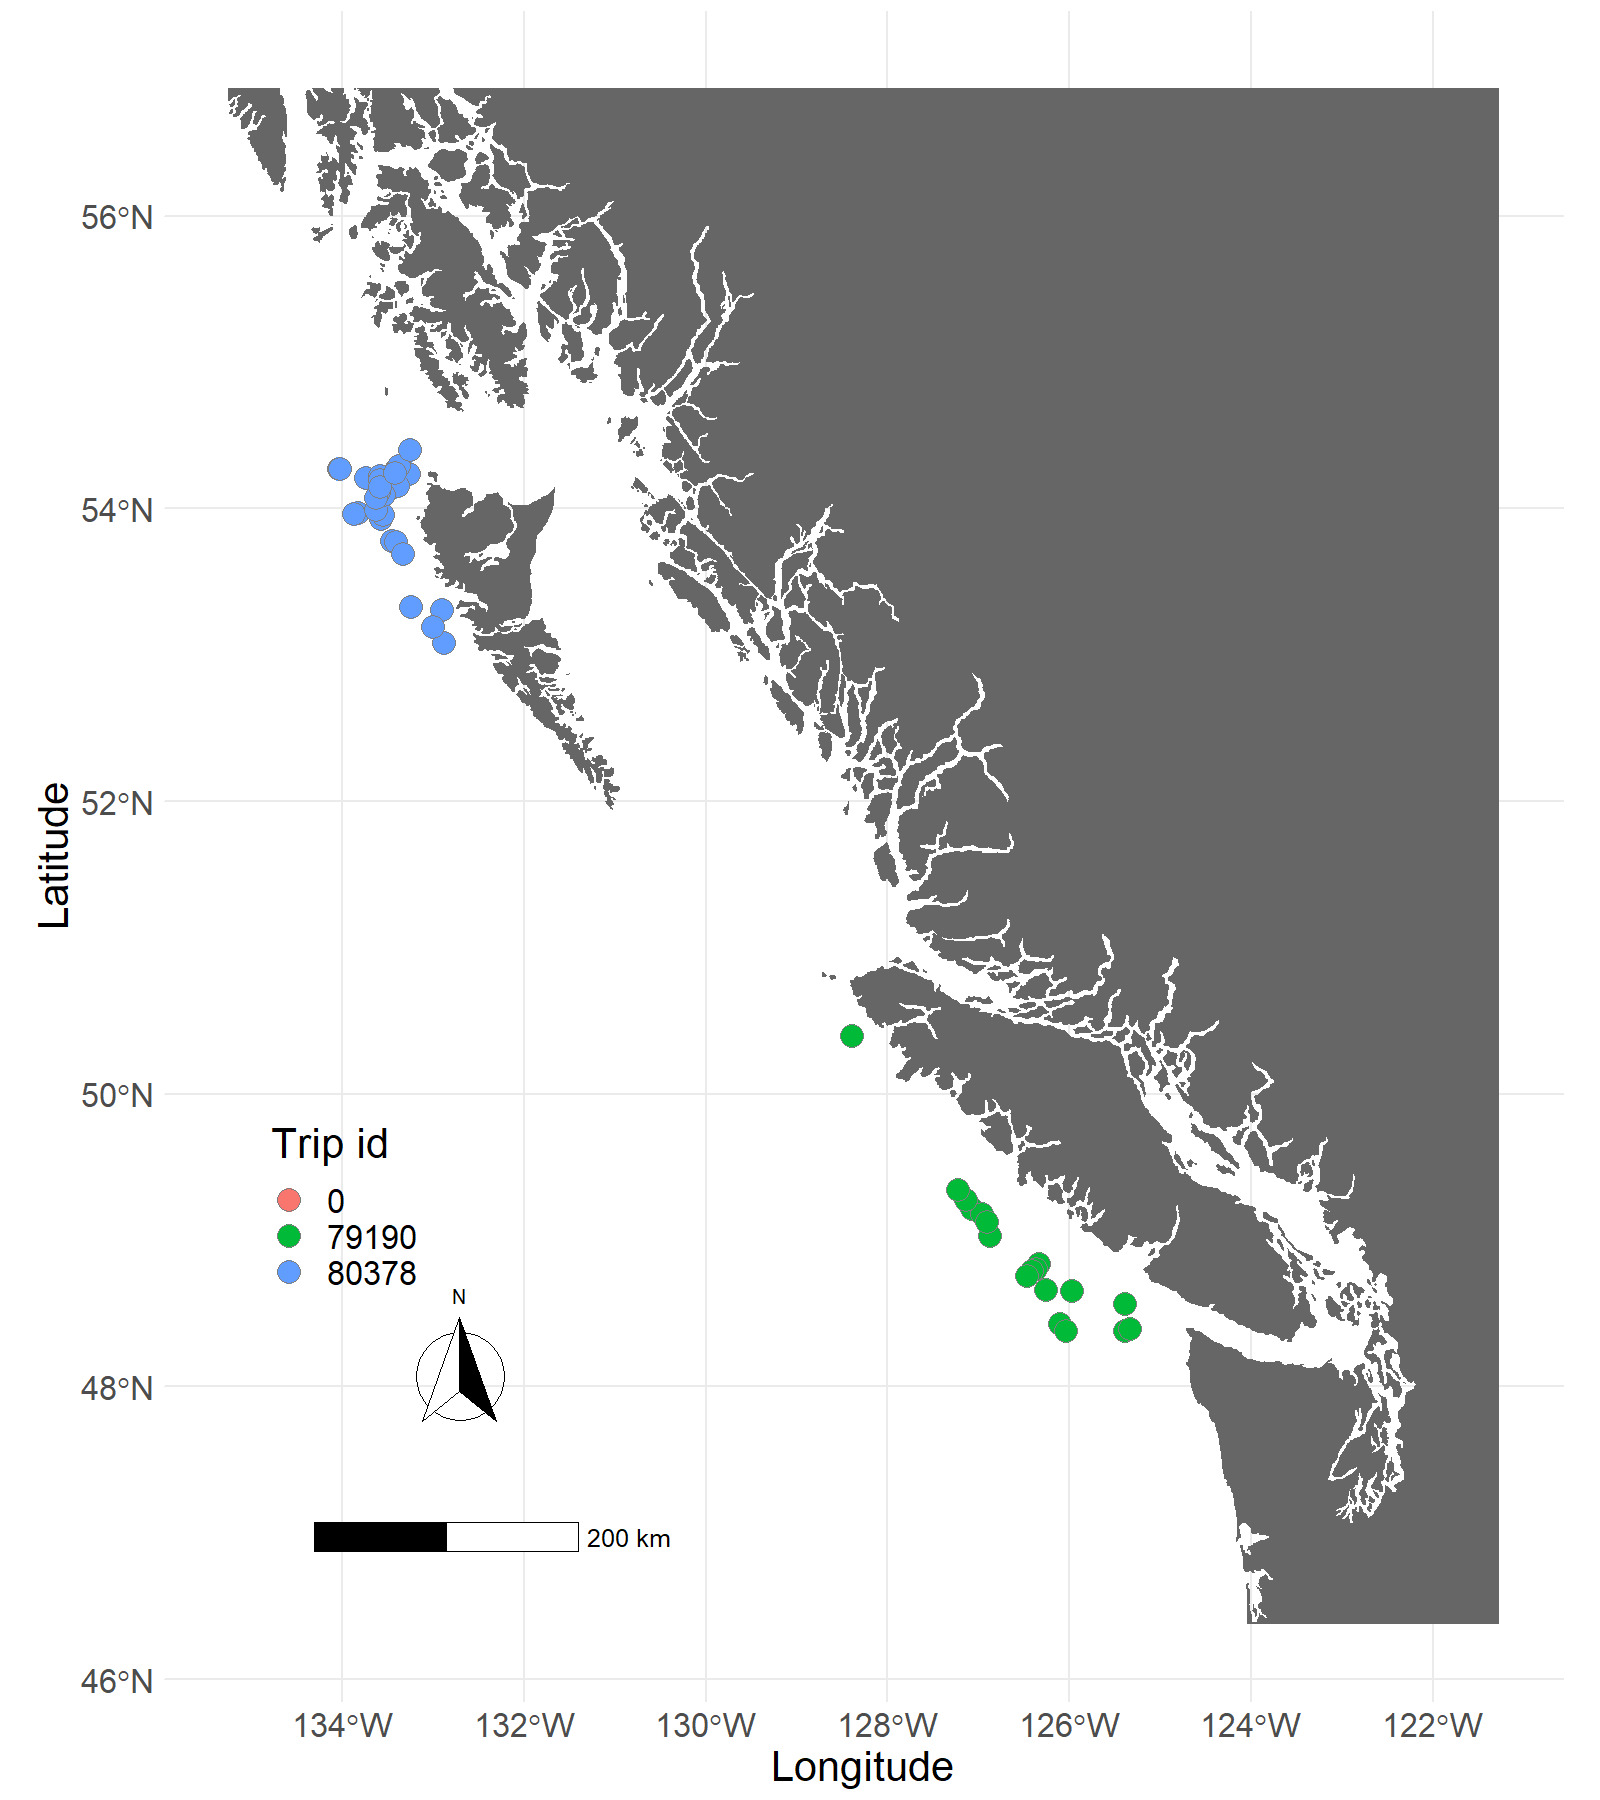
\includegraphics[width=6in]{figures/Figure1}}{Figure} 

}

\caption{Sample locations from the 2016 WCVI, 2016 WCHG research surveys and 2017 pilot study. The sample locations of the salmon survey are unknown.}\label{fig:figure1}
\end{figure}

\begin{figure}[htb]

\pdftooltip{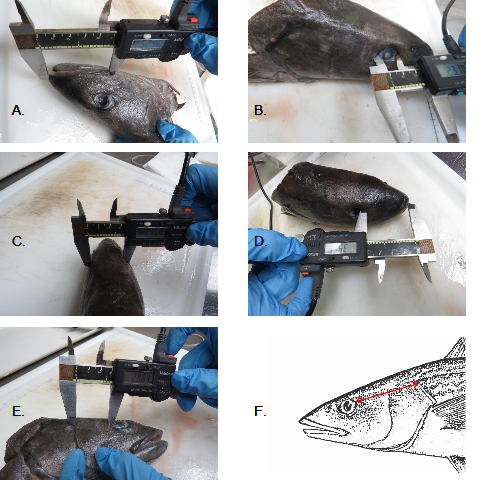
\includegraphics[width=470px]{figures/Figure2}}{Figure} \hfill{}

\caption{Relationship between cranial lengths (UJ, ED, ID) vs fork length in millimeters. Predicted points represented by black circles, measured values colored by residual scale.}\label{fig:figure2}
\end{figure}

\begin{figure}[htb]

\pdftooltip{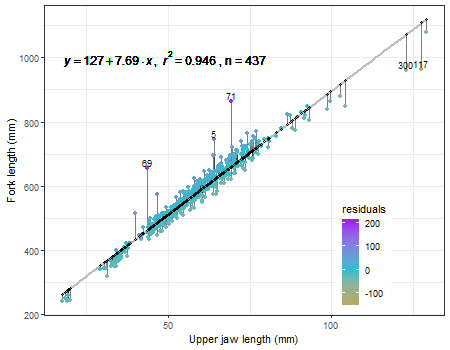
\includegraphics[width=470px]{figures/Figure3}}{Figure} \hfill{}

\caption{Relationship between cranial lengths (SL, PP, PO) vs fork length in millimeters. Predicted points represented by black circles, measured values colored by residual scale.}\label{fig:figure3}
\end{figure}
\clearpage

\begin{appendices}
\counterwithin{figure}{section}
\counterwithin{table}{section}
\counterwithin{equation}{section}

\clearpage

\section{IMAGES OF THE SIX CRANIAL DIMENSION MEASUREMENTS.}
\label{app:first-appendix}

A. Upper jaw measurement (UJ); B. Eye diameter measurement (ED); C. Interorbital distance (ID); D. Snout length (SL); E. Post orbital to preoperculum length measurement (PP); F. Post orbital head length (PO).
\begin{center}\pdftooltip{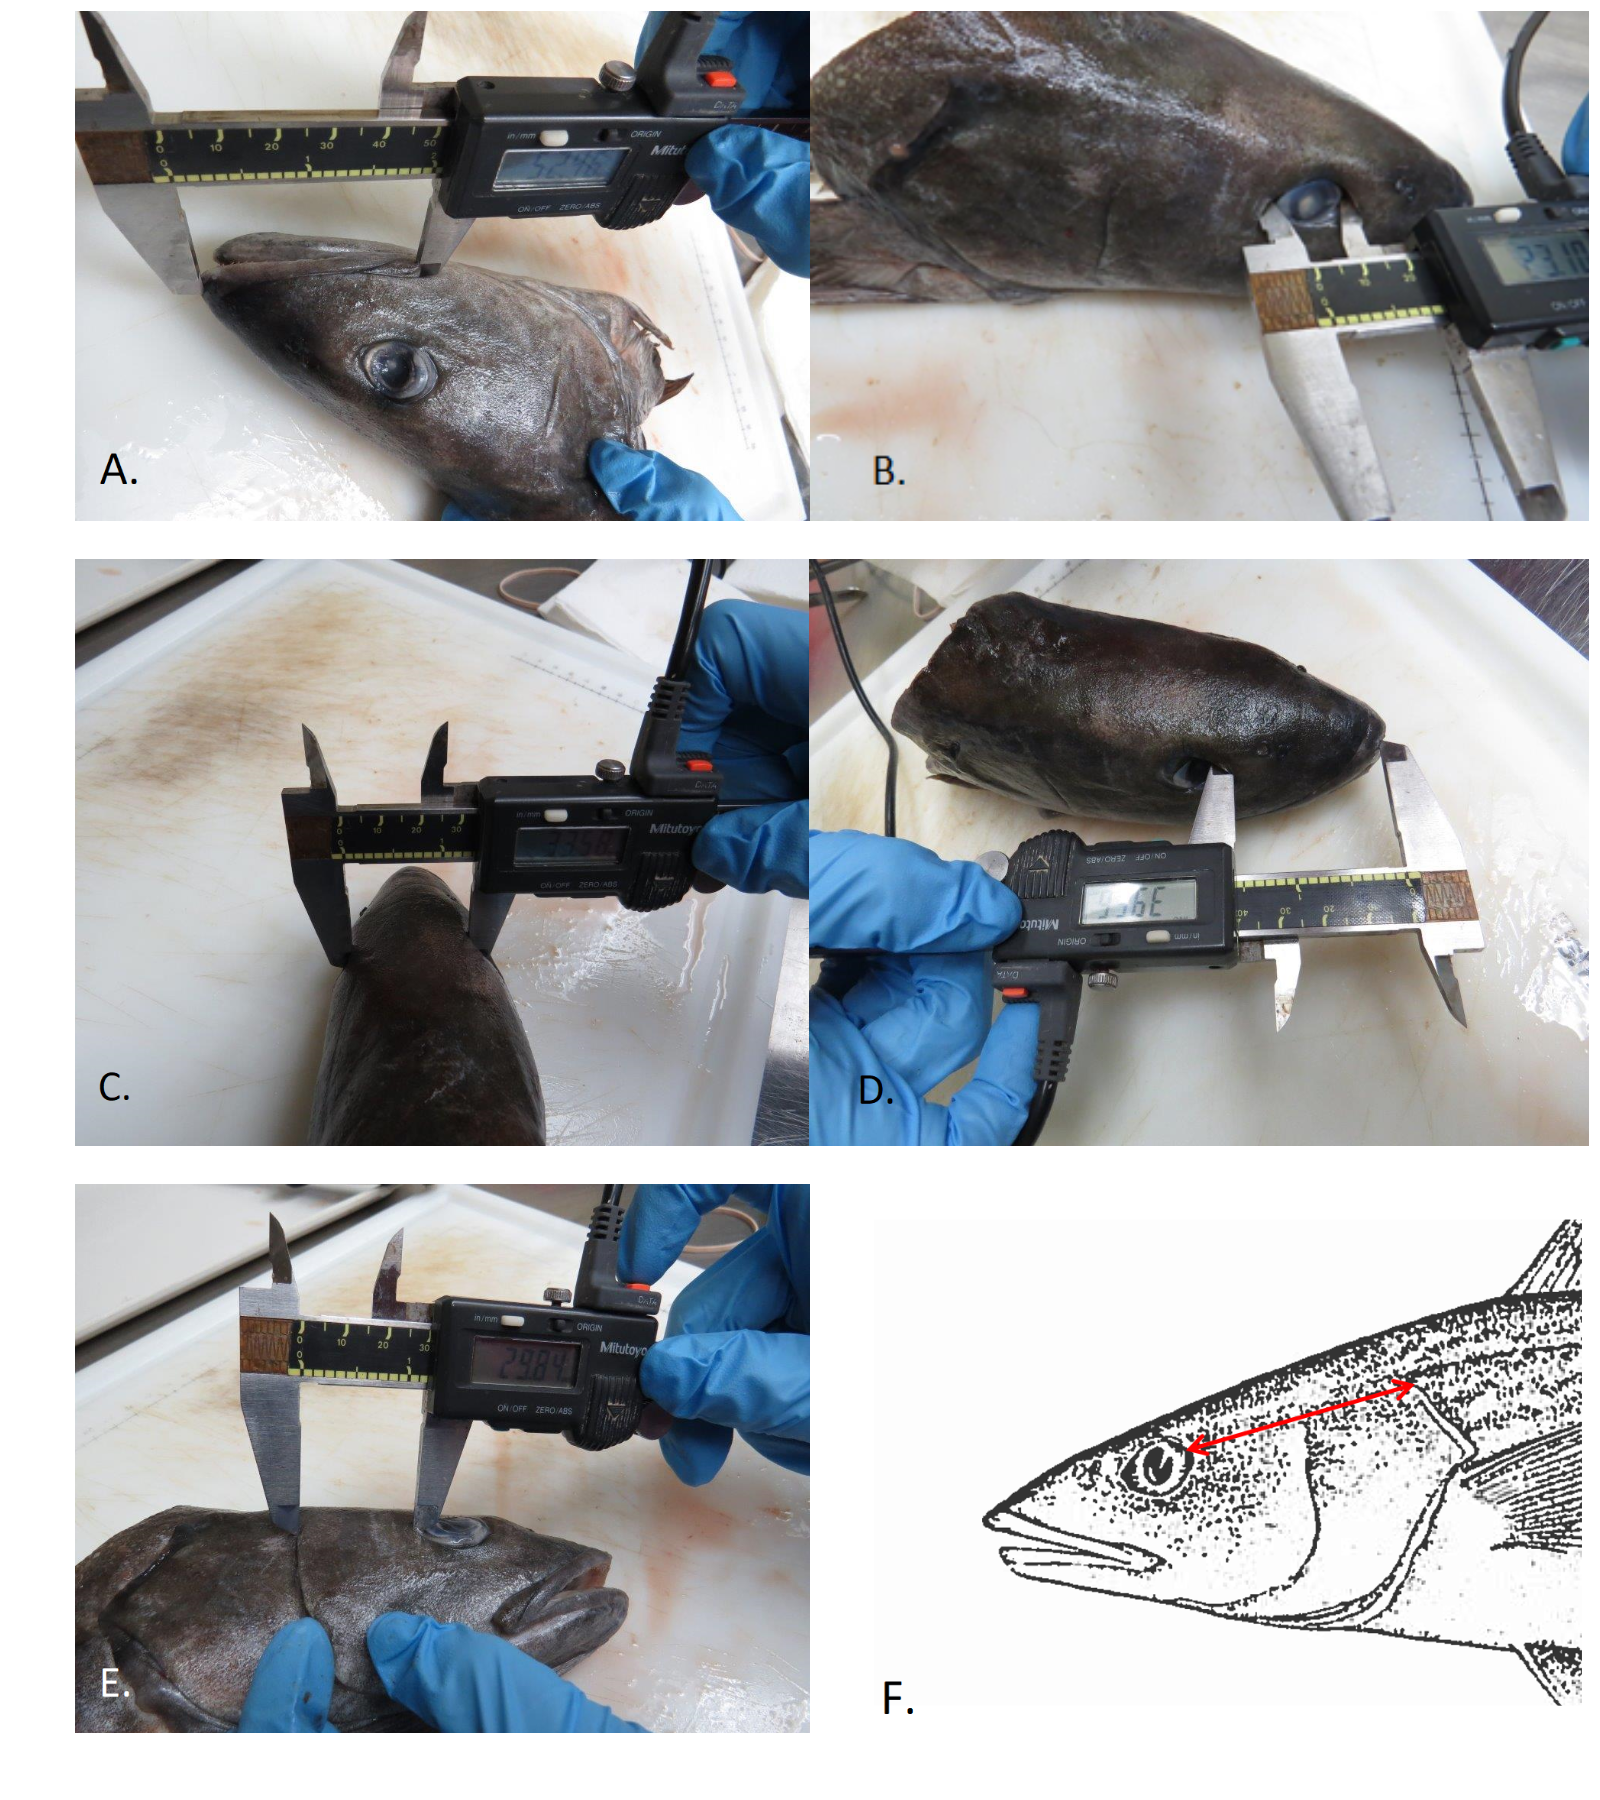
\includegraphics[width=6in]{figures/AppendixA}}{Figure} \end{center}

\clearpage

\section{SEX DETERMINATION BY OPERCULUM MARKING}
\label{app:second-appendix}

Instructions for sex determinations and operculum knife cuts for sablefish males and females.
\begin{center}\pdftooltip{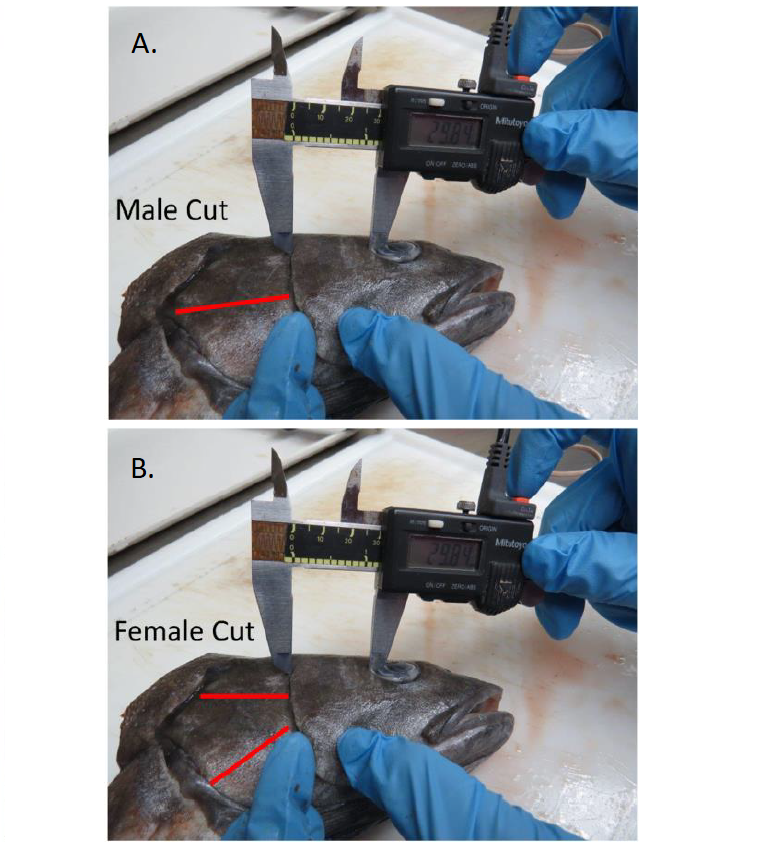
\includegraphics[width=6in]{figures/AppendixB}}{Figure} \end{center}
\clearpage

\end{appendices}

\clearpage

\hypertarget{references}{%
\section{References}\label{references}}

\noindent \vspace{-2em} \setlength{\parindent}{-0.2in} \setlength{\leftskip}{0.2in} \setlength{\parskip}{8pt}

\hypertarget{refs}{}
\begin{CSLReferences}{1}{0}
\leavevmode{\hypertarget{ref-Beamish1981}{}}%
Beamish, R., and Fournier, D.D.A. 2011. A method for comparing the precision of a set of age determinations. Canadian Journal of Fisheries and Aquatic Sciences 38: 982--983.

\leavevmode{\hypertarget{ref-Cox2019}{}}%
Cox, S.P., Holt, K., and Johnson, S. 2019. Evaluating the robustness of management procedures for the {Sablefish} (*anoplopoma fimbria*) fishery in {British Columbia, Canada} for 2017-18. DFO Can. Sci. Advis. Sec. Res. Doc. 2019/032. vi + 79 p.

\leavevmode{\hypertarget{ref-Haist2001}{}}%
Haist, R.H., V., and Wyeth, M. 2001. Sablefish {Stock Assessment} for 2001 and {Advice to Managers} for 2002. DFO Can. Sci. Advis. Sec. Res. Doc. 2001/135.

\leavevmode{\hypertarget{ref-Isermann2005}{}}%
Isermann, D.A., and Vandergoot, C.S. 2005. Predicting walleye total length from head and mandible measurements. North American Journal of Fisheries Management 25(1): 316--321. Taylor \& Francis.

\leavevmode{\hypertarget{ref-Nottingham2018}{}}%
Nottingham, M.K., Williams, D.C., Wyeth, M.R., and Olsen, N. 2018. Summary of the west coast haida gwaii synoptic bottom trawl survey, august 25 - september 26, 2016. Can. Manuscr. Rep. Fish. Aquat. Sci. 3151: viii: 51 p.

\leavevmode{\hypertarget{ref-Park2007}{}}%
Park, I.S., Kim, Y.J., Choi, H.J., Oh, S.Y., Noh, C.H., and Lee, S.H. 2007. Total length estimation from head dimensions of artificially propagated brown croaker miichthys miiuy. Korean J. Ichthyol. 19: 128--131.

\leavevmode{\hypertarget{ref-R}{}}%
R Core Team. 2021. R: A language and environment for statistical computing. R Foundation for Statistical Computing, Vienna, Austria.

\leavevmode{\hypertarget{ref-Richardson2015}{}}%
Richardson, J., Shears, N., and Taylor, R. 2015. Using relative eye size to estimate the length of fish from a single camera image. Marine Ecology Progress Series 538.

\leavevmode{\hypertarget{ref-Rondeau2013}{}}%
Rondeau, E.B., Messmer, A.M., Sanderson, D.S., Jantzen, S.G., Schalburg, K.R. von, Minkley, D.R., Leong, J.S., Macdonald, G.M., Davidsen, A.E., Parker, W.A., Mazzola, R.S.A., Campbell, B., and Koop, B.F. 2013. Genomics of sablefish (anoplopoma fimbria): Expressed genes, mitochondrial phylogeny, linkage map and identification of a putative sex gene. BMC Genomics 14(1): 452. Journal Article.

\leavevmode{\hypertarget{ref-Serafy1996}{}}%
Serafy, J.E., Schmitz, C.M., Capo, T.R., Clarke, M.E., and Ault, J.S. 1996. Total length estimation of red drum from head dimensions. The Progressive Fish-Culturist 58(4): 289--290. Taylor \& Francis.

\leavevmode{\hypertarget{ref-Shaw1997}{}}%
Shaw, W., and McFarlane, G. 1997. Development of sablefish, anoplopoma fimbira larvae off the west coast of british columbia and transformation in the juvenile stage. NOAA Tech. Rep. NMFS 130: 3--12.

\leavevmode{\hypertarget{ref-Williams2018}{}}%
Williams, D.C., Nottingham, M.K., Olsen, N., and Wyeth, M.R. 2018. Summary of the west coast vancouver island synoptic bottom trawl survey, may 24 - june 15, 2016. Can. Manuscr. Rep. Fish. Aquat. Sci. 3137: viii: 54 p.

\end{CSLReferences}
\end{document}
